\section{Atributo}
\label{sec:atributo}

Los atributos son los elementos utilizados en el standard UML para designar
propiedades que son inherentes de clases, una vez instanciados estos toman
valor y ayudan al manejo de datos del objeto, el lenguaje propuesto permite el
manejo de los atributos y algunas otras cuestiones que están relacionadas con
estos.

La definición de un atributo según notacion BNF es la siguiente:

\begin{lstlisting}[basicstyle=\footnotesize\ttfamily]
  <atributo> ::= <visibilidad> <espacio-blanco> <nombre> ":" <tipo>
\end{lstlisting}

Teniendo en cuenta que se tiene que estar en el contexto de una clase para que
el mismo tenga sentido, a continuación un ejemplo:\\

\begin{displayquote}
	\texttt{Consigna}: \textit{se desea tener una clase que permita el manejo de
	información de una persona, la información a manejar es el nombre, apellido
	y DNI}.
\end{displayquote}

Lo cual se puede representar mediante un diagrama de clase
de la siguiente manera:

\begin{figure}[H]
	\centering
	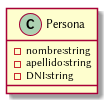
\includegraphics[width=.2\linewidth]{diagramas_clases/ej_diag_clase.png}
	\caption{Representación gráfica de la consigna mediante UML}
	\label{fig:ej_diag_clase.png}
\end{figure}

Teniendo esta información se puede armar un modelo en el lenguaje director que
concuerde con estos requerimientos. Dado a que por el momento unicamente se
está tratando con los atributos no se tendrá en cuenta la declaración de la
clase \texttt{Persona} mencionada en la consigna propuesta.

\begin{lstlisting}[label=frag:atributo]
  ...
		private nombre:string
		private apellido:string
		private DNI:string
	...
\end{lstlisting}

Lo expuesto en el \texttt{Fragmento \ref{frag:atributo}}, si bien, demuestra
la capacidad del lenguaje de describir una serie de atributos con sus
respectivos metadatos (visibilidad y tipo), también se pretende dar los
primeros pasos para la futura implementación de la compatibilización con los
futuras funcionalidades extraídas de un acercamiento al Lenguaje de
Restricción de Objetos, puesto a que la adición de funcionalidades de éstas
características automatizaria aún mas el proceso de
desarrollo y permitiría el pase de modelo-a-código de manera mas sencilla.
Las características que se implementan compatibles funcionalidades brindadas
por OCL son las de modificadores para los atributos, ademas de los mencionados
anteriormente, estos modificadores ya se mencionaron en la \texttt{Sección
\ref{sec:palabrasreservadas}}.

Como ejemplo, se podrían aplicar algunas de estas cuestiones a lo implementado
al \texttt{Fragmento \ref{frag:atributo}}.

\begin{lstlisting}[label=frag:atributo_restr]
  ...
		private nombre:string
		private apellido:string
		private DNI:string {@id, @readOnly, @unique}
	...
\end{lstlisting}

De esta forma, lo implementado en el \texttt{Fragmento
\ref{frag:atributo_restr}} brinda información como para que se pueda determinar
que el atributo DNI:
\begin{itemize}
	\item debe ser tratado como un identificador de la clase.
	\item debe ser de solo lectura, de este modo se deduce que no es necesaria la
		implementacion de un método \texttt{set} para el mismo.
	\item debe ser unico en el listado de personas, es decir, no se puede
		repetir.
\end{itemize}

Lo cual da información relevante para que la herramienta pueda brindar
resultados mas cercanos al dominio en el que se esté trabajando.

Se puede dejar expresado que el BNF, teniendo en cuenta la incorporación de lo
demostrado quedaría de la siguiente manera:

\begin{lstlisting}[basicstyle=\ttfamily\footnotesize, label=frag:bnf_atributo_restr]
		<atributo> ::= <visibilidad> <nombre> ":" <tipo>
		"{" <modificador> "}"
\end{lstlisting}

\begin{lstlisting}[language=Java, basicstyle=\tiny\ttfamily, label=frag:bnf_atributo_modif]
		<modificador> ::= @id | @readOnly | @unique | @sequence | <modificador>
\end{lstlisting}

\subsection{Autómata Finito}
\begin{figure}[H]
	\centering
	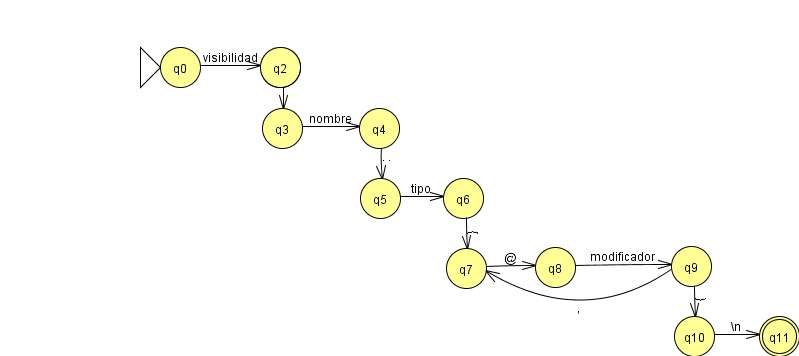
\includegraphics[width=.4\linewidth]{automatas_finitos/atributoDrt.png}
	\caption{Autómata finito para un atributo con restricciones de objeto}
	\label{fig:af_atr_modif}
\end{figure}
